\section{System overview}
\label{sec:system_overview}

Figure~\ref{fig:pipeline} summarizes Agentproof's workflow. The system ingests a
framework-specific agent definition, extracts an abstract graph model, and then
runs a suite of structural and temporal checks.

\begin{figure}[t]
  \centering
  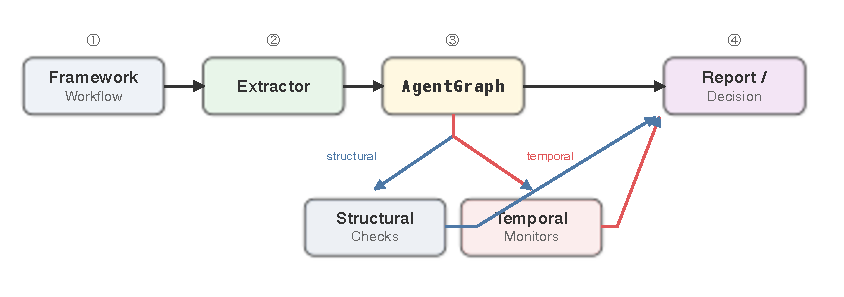
\includegraphics[width=\linewidth]{figures/pipeline.pdf}
  \caption{Agentproof pipeline: extract a framework workflow into an abstract
  graph model, run structural verification, and compile temporal policies into
  monitors for trace evaluation.}
  \label{fig:pipeline}
\end{figure}

\paragraph{Step 1: Obtain a workflow object.}
The approach targets agent orchestration libraries that expose control
flow as a graph or composition tree. Agentproof provides extractors for
LangGraph, Google ADK, AutoGen, and CrewAI
\citep{langgraph_docs,google_adk_docs,autogen_agentchat,crewai_docs}.

\paragraph{Step 2: Extract an \texttt{AgentGraph}.}
Each framework has an extractor that produces a common representation: a set of
typed nodes and typed edges with optional metadata (e.g., tool names bound to a
node). This makes downstream analyses framework-agnostic.

\paragraph{Step 3: Run structural checks.}
Structural checks detect workflow defects that do not require executing the
agent: unreachable nodes, dead ends, routing shape mismatches, and the presence
of human-in-the-loop nodes when required by policy.

\paragraph{Step 4: Compile temporal policies.}
A temporal policy DSL is compiled to DFAs. Policies are written against
abstract events (tool calls, action tags, or decisions) rather than
framework internals.

\paragraph{Step 5: Evaluate monitors over traces.}
Monitors are evaluated over offline simulated traces or integrated into
a runtime event stream. Violations are mapped to handling levels (warn,
block, halt, escalate) to support different operational postures.

